\section{ Live Variabl Analysis   }

In compilers, live variable analysis (or simply liveness analysis)
is a classic data-flow analysis to calculate the variables that
are live at each point in the program. A variable is live at
some point if it holds a value that may be needed in the future,
or equivalently if its value may be read before the next time
the variable is written to. \footnote{based on Wikipedia}

\subsection{Motivation}

Programs may contain

\begin{itemize}
	\item code which gets executed but which has no useful
	      effect on the program's overall result;
	\item occurrences of variables being used before they
	      are defined;\footnote{we can use liveness information to find undefined variables.}
	\item many variables which need to be allocated
	      registers and/or memory locations for compilation.\footnote{Two	variables	can	use	the	same	register	if	they	are	never	in	use	at	the
		      same time(i.e,	never	simultaneously live). Register	allocation
		      uses liveness information.}

\end{itemize}

The concept of variable liveness is useful in dealing
with all three of these situations.


Liveness analysis is highly used for \textbf{register allocation}(If variable \texttt{x} is live in a basic block b, it is a potential candidate for
register allocation) and \textbf{dead code elimination}(If variable \texttt{x} is not live after an assignment \texttt{x =...}, then the assignment is
redundant and can be deleted as dead code).


\subsection{Problem formulation}
Liveness is a data-flow property of variables:
“Is the value of this variable needed?” We therefore
usually consider liveness from an instruction's
perspective: each instruction (or node of the
flowgraph) has an associated set of live variables.


\subsection{Semantic vs. syntactic}


There are two kinds of variable liveness : Semantic liveness and Syntactic liveness.


A variable x is \textbf{semantically} live at a node n if there is
some execution sequence starting at n whose (externally
observable) behaviour can be affected by changing the
value of x. Semantic liveness is concerned with
the execution behaviour of the program.

A variable is \textbf{syntactically} live at a node if there is a
path to the exit of the flow graph along which its
value may be used before it is redefined. Syntactic liveness is concerned with properties of
the syntactic structure of the program.


So what is the difference between Semantic liveness and Syntactic liveness? syntactic liveness
is a computable approximation of semantic liveness.


Consider the example \ref{lst:expr2}


\begin{lstlisting}[language=C,frame=single, caption=An example to illustrate semantic syntatic,label = lst:expr2]
    int t = x * y;
    if ((x+1)*(x+1) == y) {
     t = 1;
    }
    if (x*x + 2*x + 1 != y) {
     t = 2;
    }
    return t;
\end{lstlisting}

In fact, t is dead in node \texttt{int t = x * y;} because one of the conditions will be true,
so on every execution path t is redefined before it is returned.
The value assigned by the first instruction is never used.


But on read path from Figure \ref{fig:liveex} through the
flowgraph, t is not
redefined before it's used,
so t is syntactically live at
the first instruction.Note that this path never
actually occurs during
execution.

\begin{figure}[h]
	\centering
	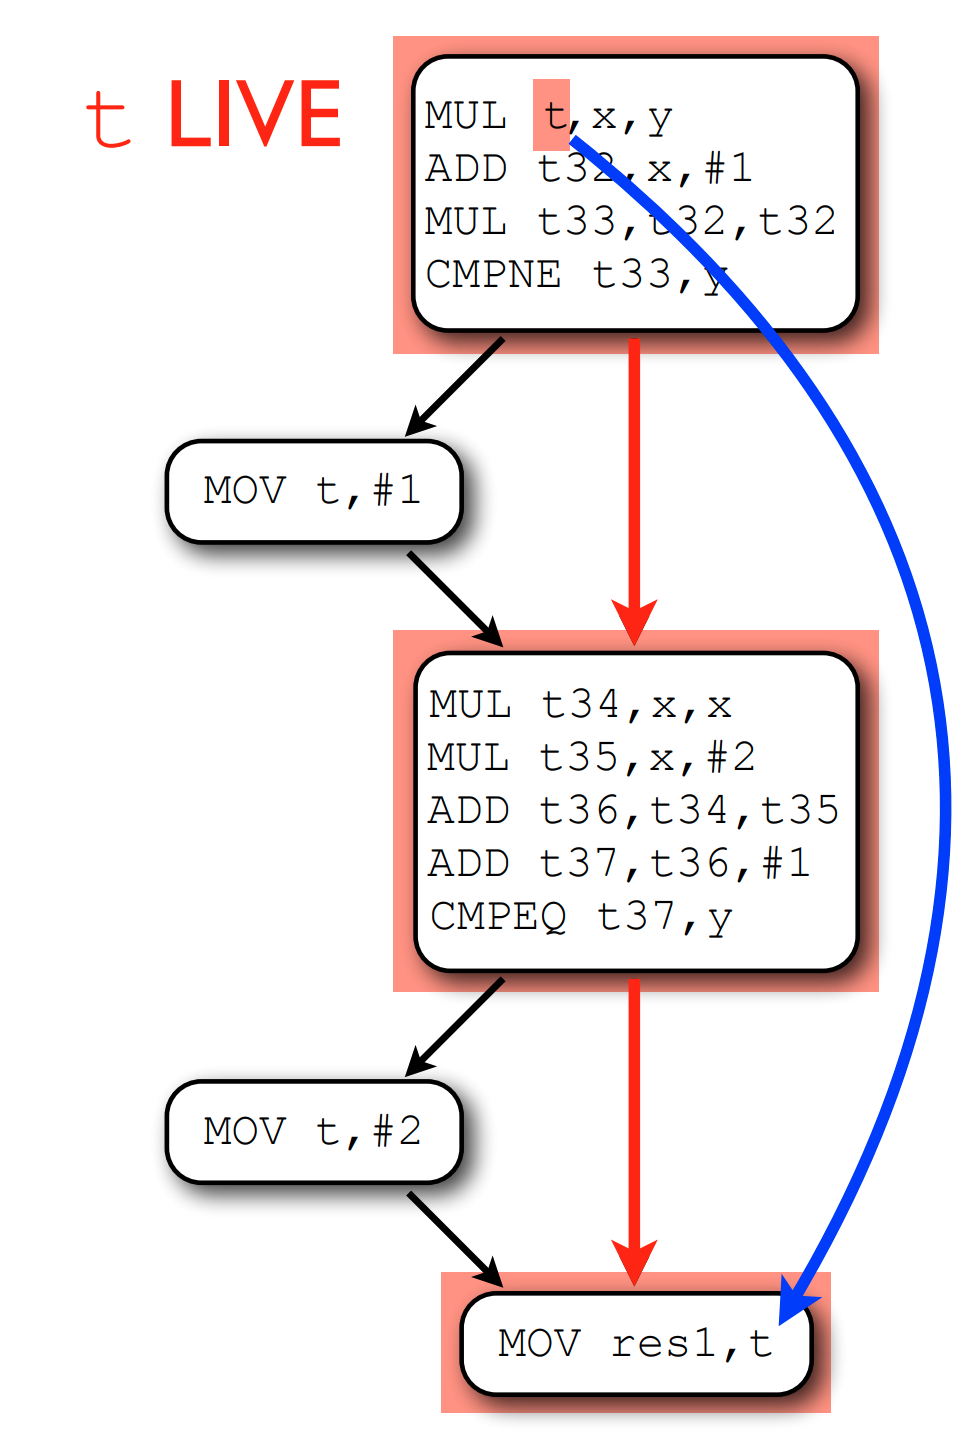
\includegraphics[width=0.3\textwidth]{liveex.png}
	\caption{CFG for \ref{lst:expr2}}
	\label{fig:liveex}
\end{figure}


\subsection{Summary}


\begin{center}
	\begin{tabular}{|c|c|}
		\hline Direction                         & Backward                                            \\
		\hline Domain                            & Sets	of	variables                                     \\
		\hline Meet operator                     & \( \cup \)                                          \\
		\hline Top(T)                            & $\phi$                                              \\
		\hline Bottom                            & Universal Set                                       \\
		\hline Boundary condition                & $\mathrm{IN[EXIT]} = \phi$                          \\
		\hline Initialization for internal nodes & $\mathrm{IN[B]} = \phi$                             \\
		\hline Finited escending chain?          & \checkmark                                          \\
		\hline Transfer function                 & $f_b(x) = \mathrm{USE}_b \cup (x - \mathrm{DEF}_b)$ \\
		\hline Monotone\&Distributive?           & \checkmark                                          \\
		\hline
	\end{tabular}
\end{center}




\subsection{Strongly Live Variables Analysis\cite{LiveVari29:online}}

A variable is strongly live if
\begin{itemize}

	\item it is used in a statement other than assignment statement, or
	      (same as simple liveness)
	\item it is used in an assignment statement defining a variable that is
	      strongly live
\end{itemize}


\begin{figure}[H]
	\centering
	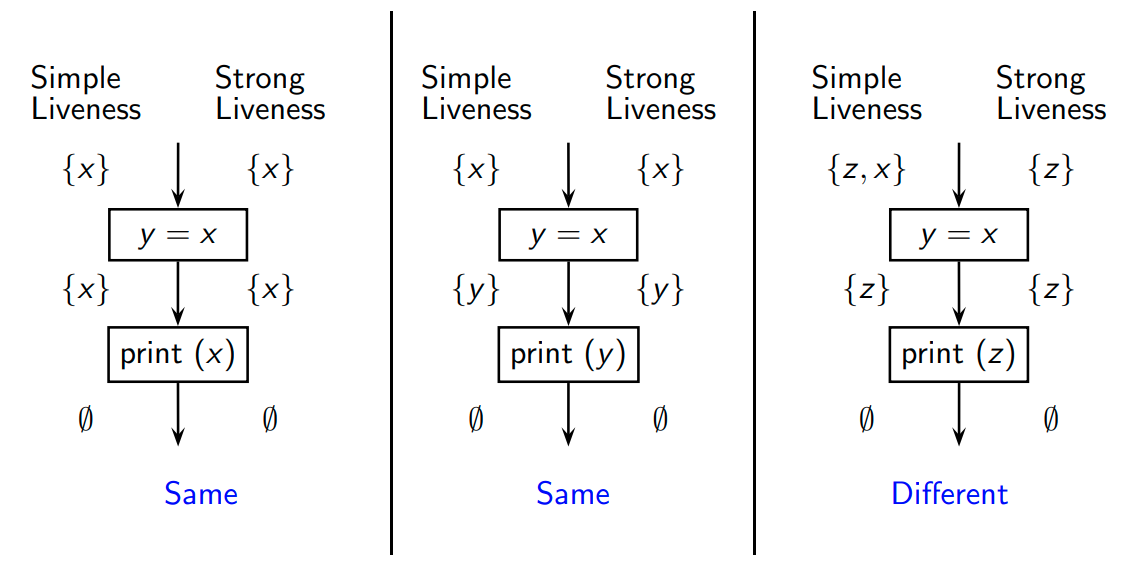
\includegraphics[width=0.7\textwidth]{p217.png}
	\caption{Understanding Strong Liveness}
	\label{fig:p217}
\end{figure}


A variable is live at a program
point if its current value is likely
to be used later. We want to compute the smallest
set of variables that are live. Simple liveness considers every
use of a variable as useful. Strong liveness checks the liveness
of the result before declaring the
operands to be live. Strong liveness is more precise
than simple liveness. The transfer function of Strongly Live Variables Analysis is shwon
below:


$$
	f_n(X)= \begin{cases}(X-\{y\}) \cup(Opd(e) \cap \mathbb{V}ar) & n \text { is } y=e, e \in \mathbb{E}pr, y \in X \\ X-\{y\} & n \text { is input }(y) \\ X \cup\{y\} & n \text { is use }(y) \\ X & \text { otherwise }\end{cases}
$$


The first case means that If \texttt{y} is not strongly live, the
assignment is skipped using
the “otherwise” clause

\begin{figure}[H]
	\centering
	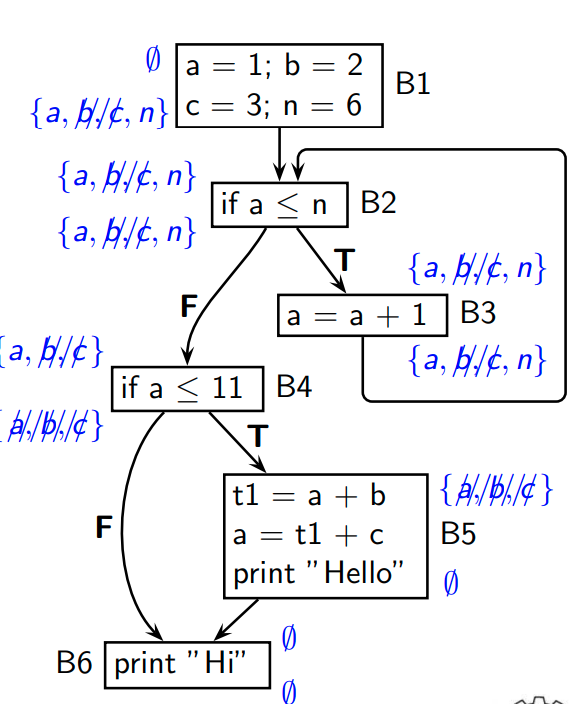
\includegraphics[width=0.4\textwidth]{p218.png}
	\caption{Simple Liveness VS. Strong Liveness.}
	\label{fig:p218}
\end{figure}
